\section{Neo4J}

\begin{itemize}
    \item Daten werden in Form von Knoten gespeichert, die von einem gewissen Typen sein können (z.B. Person)
    \item Knoten werden über Kanten verbunden, welche ebenfalls einem Typen + gewisse Attribute haben können
\end{itemize}
\subsection{Befehle}
\subsubsection{Daten einspielen}
\begin{figure}[H]
    \centering
    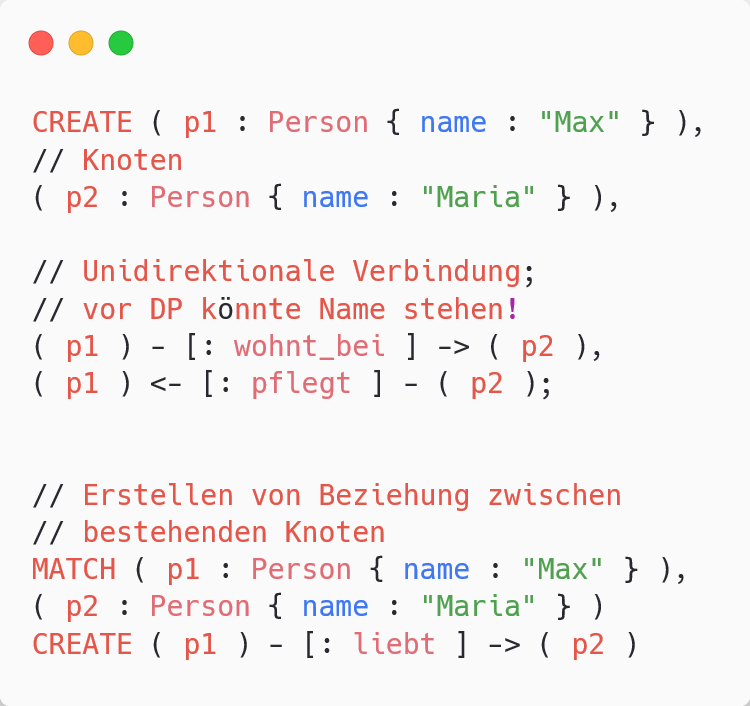
\includegraphics[scale=.2]{res/themenkorb_8/cypher_insert.png}
\end{figure}
\subsubsection{Daten updaten}
\begin{figure}[H]
    \centering
    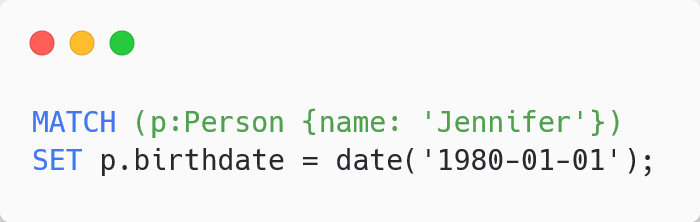
\includegraphics[scale=.3]{res/themenkorb_8/cypher_update.png}
\end{figure}
\subsubsection{Daten löschen}
\begin{figure}[H]
    \centering
    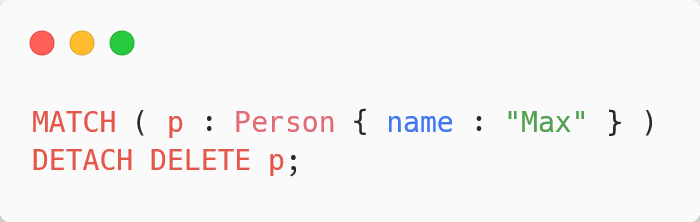
\includegraphics[scale=.3]{res/themenkorb_8/cypher_delete.png}
\end{figure}
\subsubsection{Daten anzeigen}
\begin{figure}[H]
    \centering
    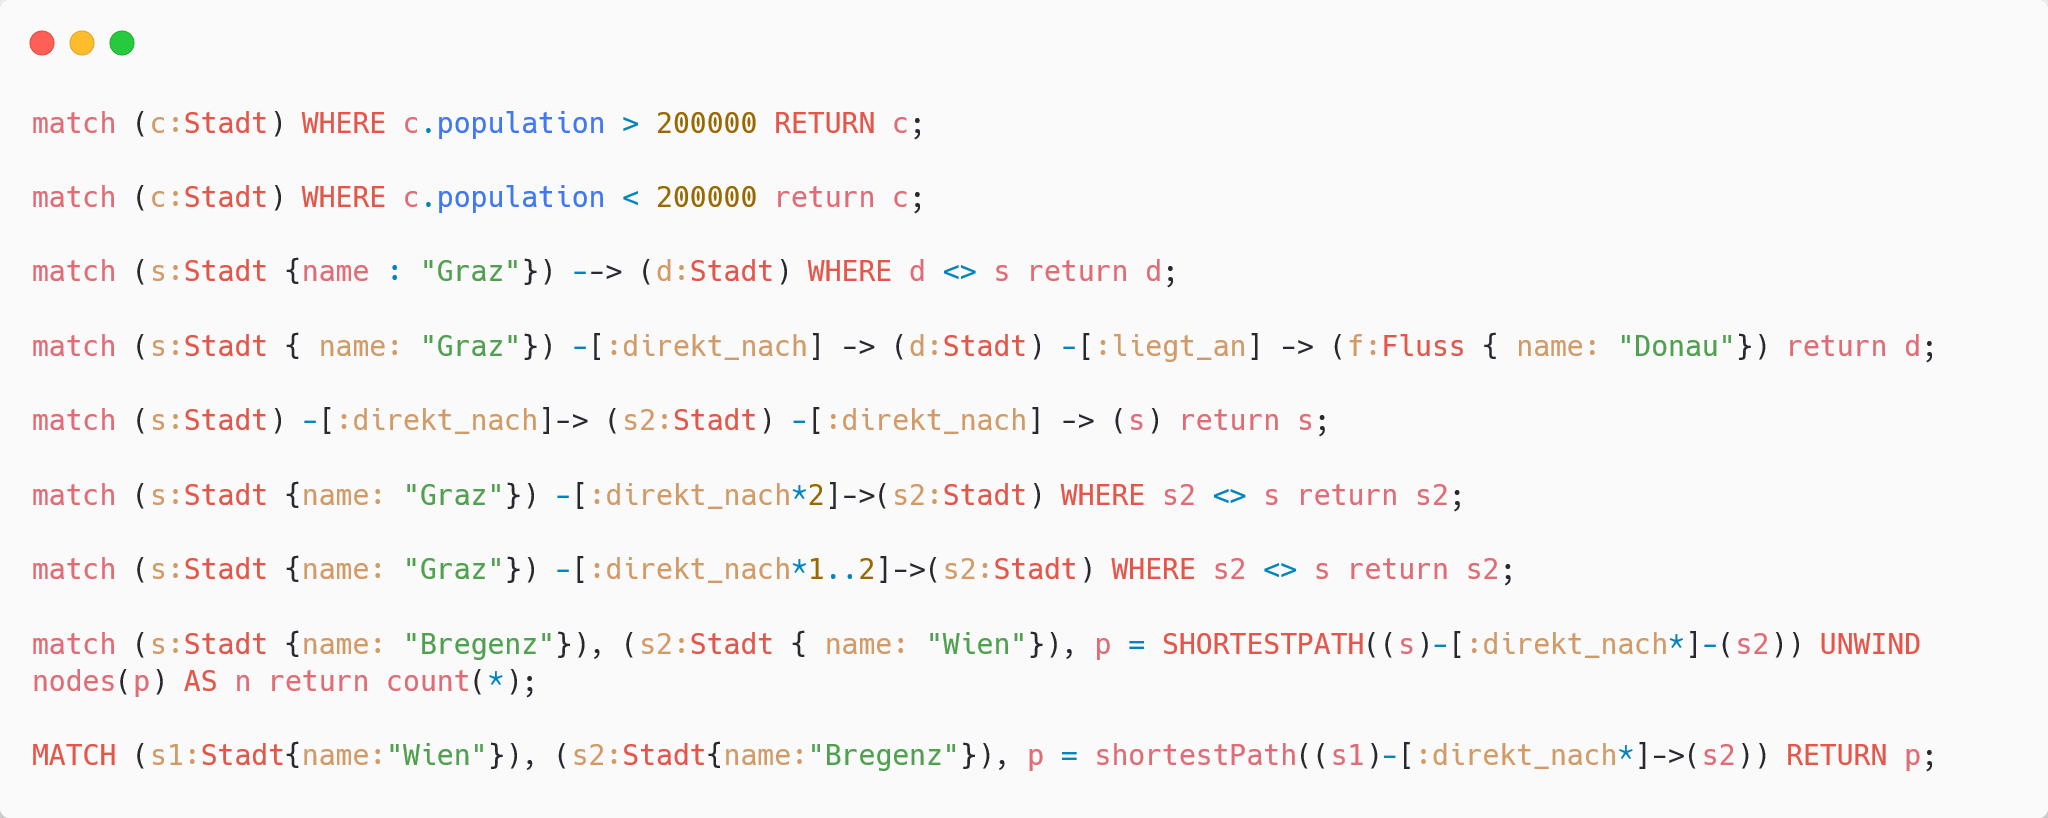
\includegraphics[width=\textwidth]{res/themenkorb_8/cypher_view.png}
\end{figure}